\documentclass[ucs,10pt]{beamer}
 
% Template for talks using the Logo of STCE and Corporate Design of RWTH Aachen
% adapted from:
% https://www.mi.fu-berlin.de/w/Mi/BeamerTemplateCorporateDesign

\usepackage{amsmath,dsfont,listings}
% ** for picture **
\usepackage{graphicx}

%%% STCE logo
% small version for upper right corner of normal pages
\pgfdeclareimage[height=0.9cm]{university-logo}{rwth_i12_softw-werkz_en_rgb.png}
\logo{\pgfuseimage{university-logo}}
% large version for upper right corner of title page
\pgfdeclareimage[height=1cm]{big-university-logo}{rwth_i12_softw-werkz_en_rgb.png}
\newcommand{\titleimage}[1]{\pgfdeclareimage[height=2cm]{title-image}{#1}}
\titlegraphic{\pgfuseimage{title-image}}
%%% end STCE logo

% NOTE: 1cm = 0.393 in = 28.346 pt;    1 pt = 1/72 in = 0.0352 cm
\setbeamersize{text margin right=3.5mm, text margin left=7.5mm}  % text margin

% colors to be used
\definecolor{text-grey}{RGB}{51, 51, 51} % grey text on white background
\definecolor{bg-grey}{rgb}{0.66, 0.65, 0.60} % grey background (for white text)
\definecolor{rwth-blue}{RGB}{0, 83, 159} % blue text
\definecolor{rwth-green}{RGB}{153, 204, 0} % green text
\definecolor{rwth-red}{RGB}{204, 0, 0} % red text (used by \alert)

% switch off the sidebars
% TODO: loading \useoutertheme{sidebar} (which is maybe wanted) also inserts
%   a sidebar on title page (unwanted), also indents the page title (unwanted?),
%   and duplicates the navigation symbols (unwanted)
\setbeamersize{sidebar width left=0cm, sidebar width right=0mm}
\setbeamertemplate{sidebar right}{}
\setbeamertemplate{sidebar left}{}
%    XOR
% \useoutertheme{sidebar}

% frame title
% is truncated before logo and splits on two lines
% if neccessary (or manually using \\)
\setbeamertemplate{frametitle}{%
    \vskip-30pt \color{purple}\large%
    \begin{minipage}[b][23pt]{80.5mm}%
    \flushleft\insertframetitle%
    \end{minipage}%
}

%%% title page
% TODO: get rid of the navigation symbols on the title page.
%   actually, \frame[plain] *should* remove them...
\setbeamertemplate{title page}{
% upper right: STCE logo
\vskip2pt\hfill\pgfuseimage{big-university-logo} \\
\vskip6pt\hskip3pt
% title image of the presentation
% set the title and the author
\begin{center}
\vskip4pt
\large \inserttitle \vskip5pt  \small \insertsubtitle
\vskip8pt
	\normalsize \insertauthor %\\ 
	%\includegraphics[width=2cm]{../../foto_naumann}	
\\ [5mm]
	\footnotesize \insertinstitute 
\end{center}
}
%%% end title page

%%% colors
\usecolortheme{lily}
\setbeamercolor*{normal text}{fg=black,bg=white}
\setbeamercolor*{alerted text}{fg=rwth-red}
\setbeamercolor*{example text}{fg=rwth-green}
\setbeamercolor*{structure}{fg=rwth-blue}

\setbeamercolor*{block title}{fg=white,bg=black!50}
\setbeamercolor*{block title alerted}{fg=white,bg=black!50}
\setbeamercolor*{block title example}{fg=white,bg=black!50}

\setbeamercolor*{block body}{bg=black!10}
\setbeamercolor*{block body alerted}{bg=black!10}
\setbeamercolor*{block body example}{bg=black!10}

\setbeamercolor{bibliography entry author}{fg=rwth-blue}
% TODO: this doesn't work at all:
\setbeamercolor{bibliography entry journal}{fg=text-grey}

\setbeamercolor{item}{fg=rwth-blue}
\setbeamercolor{navigation symbols}{fg=text-grey,bg=bg-grey}
%%% end colors

%%% headline
\setbeamertemplate{headline}{
\vskip4pt\hfill\insertlogo\hspace{3.5mm} % logo on the right

\vskip6pt\color{rwth-blue}\rule{\textwidth}{0.4pt} % horizontal line
}
%%% end headline

%%% footline
\newcommand{\footlinetext}{\insertshortinstitute, \insertshorttitle}
\setbeamertemplate{footline}{
\vskip5pt\color{rwth-blue}\rule{\textwidth}{0.4pt}\\ % horizontal line
\vskip2pt
\makebox[123mm]{\hspace{7.5mm}
\color{rwth-blue}\footlinetext
\hfill \raisebox{-1pt}{\usebeamertemplate***{navigation symbols}}
\hfill \insertframenumber}
\vskip4pt
}
%%% end footline

%%% settings for listings package
\lstset{extendedchars=true, showstringspaces=false, basicstyle=\footnotesize\sffamily, tabsize=2, breaklines=true, breakindent=10pt, frame=l, columns=fullflexible}
\lstset{language=C++} % this sets the syntax highlighting
\lstset{mathescape=true} % this switches on $...$ substitution in code
% enables UTF-8 in source code:
\lstset{literate={ä}{{\"a}}1 {ö}{{\"o}}1 {ü}{{\"u}}1 {Ä}{{\"A}}1 {Ö}{{\"O}}1 {Ü}{{\"U}}1 {ß}{\ss}1}
%%% end listings
  

\begin{document}
\title[{\tt info@stce.rwth-aachen.de}]{\textcolor{rwth-blue}{Software Lab Computational Engineering Science} \vspace{.2cm} \\ {\small Group 12, Exception Handling}}
\author[Group 12)]{Aaron Floerke, Arseniy Kholod, Xinyang Song and Yanliang Zhu} 
\institute[Software Lab CES]{
{Informatik 12: Software and Tools for Computational Engineering (STCE)} \\ RWTH Aachen University \vspace{.5cm}
}
\date[]{24.06.2024}

\begin{frame}[plain]
\titlepage
\end{frame}

\begin{frame}
	\frametitle{Contents}
\tableofcontents
\end{frame}

\section{Preface}

\begin{frame}
\frametitle{Preface \\
	\small \color{rwth-blue} Exception Handling}

	\begin{itemize}
		\item Software always has a working domain.
		\item User of the software is not aware of all limitations.
		\item Software developer helps user by introducing appropriate exception handling.
		\item Our task is to introduce an exception handling to cppNum v2.4 and v2.5.
	\end{itemize}
\end{frame}

\section{Analysis}

\subsection{User Requirements}

\begin{frame}
\frametitle{Analysis \\
	\small \color{rwth-blue} User Requirements}
	\begin{itemize}
		\item Extend cppNum v2.4 and v2.5 with appropriate C++ exception handling.
		\item Desing at least three scalable sufficiently distinct case studies.
		\item Compare general behavior and run times with the exception handling-free version.
	\end{itemize}
\end{frame}

\subsection{fisch}

\begin{frame}
\frametitle{Analysis \\
	\small \color{rwth-blue} Definition Exception Handling}
	\begin{itemize}
		\item Exception handling is a programming concept used to manage errors and unusual conditions that arise during program execution. It allows for controlled responses to errors, ensuring the program can handle them gracefully without crashing. Key components include try, catch (or except), and finally blocks. (ChatGPT)
	\end{itemize}
\end{frame}

\subsection{System Requirements}

\begin{frame}
\frametitle{Analysis \\
	\small \color{rwth-blue} System Requirements}
	Functional:
	\begin{itemize}
		\item \textbf{Exception Handling:}
		\begin{itemize}
			\item An exception is thrown, if the system is not able to produce the correct result
			\item An exception is thrown when the system behaves in an unintended way. 
                \item An exception should be handled in such a way, as to prevent a potential crash of the system, if possible.
			\item The system must integrate C++ exception handling mechanisms in cppNum versions v2.4 and v2.5.
			\item The system must log all exceptions with appropriate error messages.
                \item A thrown exception should enhance the users ability to find bugs.
		\end{itemize}
		\item \textbf{Case Studies:}
		\begin{itemize}
			\item The system must implement at least three scalable and distinct case studies to test the modified cppNum library.
			\item Each case study must include a specific scenario that can trigger exceptions.
		\end{itemize}
		\item \textbf{Performance Comparison:}
		\begin{itemize}
			\item The system must compare the general behavior and run times of the modified cppNum versions with the original exception-free versions.
			\item The comparison results must be documented and include detailed performance metrics.
		\end{itemize}
	\end{itemize}
\end{frame}

\begin{frame}
\frametitle{Analysis \\
	\small \color{rwth-blue} System Requirements}
	Nonfunctional:
	\begin{itemize}
		\item \textbf{Exception Structure:}
		\begin{itemize}
			\item An exception is a class object.
			\item All cppNum exception classes have a single parent class to provide a clear structure.
			\item All exception classes are inherited from std::exception to catch together with other exceptions, potentially generated by third-party libraries.
		\end{itemize}
             \item \textbf{Exception Logic:}
		\item \textbf{Performance:}
		\begin{itemize}
			\item The system must ensure that the overhead introduced by exception handling is minimized.
			\item The system should not degrade the performance of cppNum versions v2.4 and v2.5 by more than 10%.
		\end{itemize}
		\item \textbf{Reliability:}
		\begin{itemize}
			\item The system must handle exceptions gracefully to prevent crashes and ensure smooth operation.
			\item The system must be able to recover from exceptions and continue processing if possible.
		\end{itemize}
        \end{itemize}
\end{frame}

\begin{frame}
\frametitle{Analysis \\
	\small \color{rwth-blue} System Requirements}
	\begin{itemize}	
            \item \textbf{Usability:}
		\begin{itemize}
			\item The system must provide clear and informative error messages to users when exceptions occur.
			\item The system should document the scenarios under which exceptions are raised and how they are handled.
		\end{itemize}
		\item \textbf{Maintainability:}
		\begin{itemize}
			\item The code implementing exception handling must be well-documented and follow coding standards.
			\item The system must use modular and clean code to facilitate future updates and maintenance.
		\end{itemize}
		\item \textbf{Scalability:}
		\begin{itemize}
			\item The system must be able to handle large datasets and complex computations in the case studies without significant performance degradation.
			\item The system must be designed to easily incorporate additional case studies in the future.
		\end{itemize}
	\end{itemize}
\end{frame}

\begin{frame}
\frametitle{Design \\
	\small \color{rwth-blue} Principal Components and Third-Party Software}
	\begin{itemize}
		\item std::exception to enherit exception classes from.
		\item Eigen library to prove applicability of LU and LLT decompositions.
		\item throw and try-catch mechanism to throw and catch exceptions.
	\end{itemize}
\end{frame}

\subsection{Class Model(s)}

\begin{frame}
\frametitle{Design \\
	\small \color{rwth-blue} Class Model(s)}
\end{frame}





\section{Implementation}

\subsection{Development Infrastructure}

\begin{frame}
\frametitle{Implementation \\
	\small \color{rwth-blue} Development Infrastructure}
	\begin{itemize}	
            \item \textbf{1.Operating System:}
				\begin{itemize}
					\item Xubuntu
				\end{itemize}
            \item \textbf{2.Programming Language and Compiler:}
				\begin{itemize}
					\item Programming Language: C++.
					\item Compiler: GCC .
				\end{itemize}
			\item \textbf{3.Libraries:}
				\begin{itemize}
					\item Eigen: A C++ library for linear algebra, providing efficient matrix and vector operations.
					\item AD: Provide a complete C++ solution for implementing algorithmic differentiation in numerical computations. 
				\end{itemize}
			\item \textbf{4. Version Control System:}
				\begin{itemize}
				\item GitHub Remote code repositories for team collaboration, code reviews, and version control. (https://github.com/ArseniyKholod/stce_ss24_ex12)
				\end{itemize}
			\item \textbf{5.Frameworks:}
					\item Doxygen: Used for generating project documentation, helping the team understand and maintain the code better.
					\item Makefile: For build management.
	\end{itemize}
\end{frame}

\subsection{Source Code}

\begin{frame}
\frametitle{Implementation \\
	\small \color{rwth-blue} Source Code}
\end{frame}

\subsection{Software Tests}

\begin{frame}
\frametitle{Implementation \\
	\small \color{rwth-blue} Software Tests}
\end{frame}



\section{Project Management}

\begin{frame}
\frametitle{Project Management \\
	\small \color{rwth-blue} Task}
	\begin{itemize}	
            \item \textbf{1.Self-study course:}
				\begin{itemize}
					\item Read source code.
					\item Discuss problems in group in Discord.
				\end{itemize}
			\item \textbf{Extend cppNum with exception handling:}
				\begin{itemize}
					\item Classification of Exceptions
					\item Add exception classes as specified in the class diagram and in alignment with the standard exception library
					\item Couple Exception Classes with Original Program
				\end{itemize}
			\item \textbf{3.Design scalable case studies:}
				\begin{itemize}
				\item Implent new cases
				\item Add timing and plotting method
				\item Test and Debug
				\end{itemize}
			\item \textbf{4.Run time difference Analysis}
			\item \textbf{5.Design scalable case studies:}
				\begin{itemize}
				\item Analysis (user requirements , use case)
				\item Source code and design
				\item Project management and live-demo(test)
				\item Case study(example) and run time analysis
				\end{itemize}
			\item *The following page of the PDF outlines the responsibilities of each person.
	\end{itemize}
\end{frame}

\begin{frame}
\frametitle{Project Management \\
    \small \color{rwth-blue} Gantt Chart}
    
    \begin{center}
        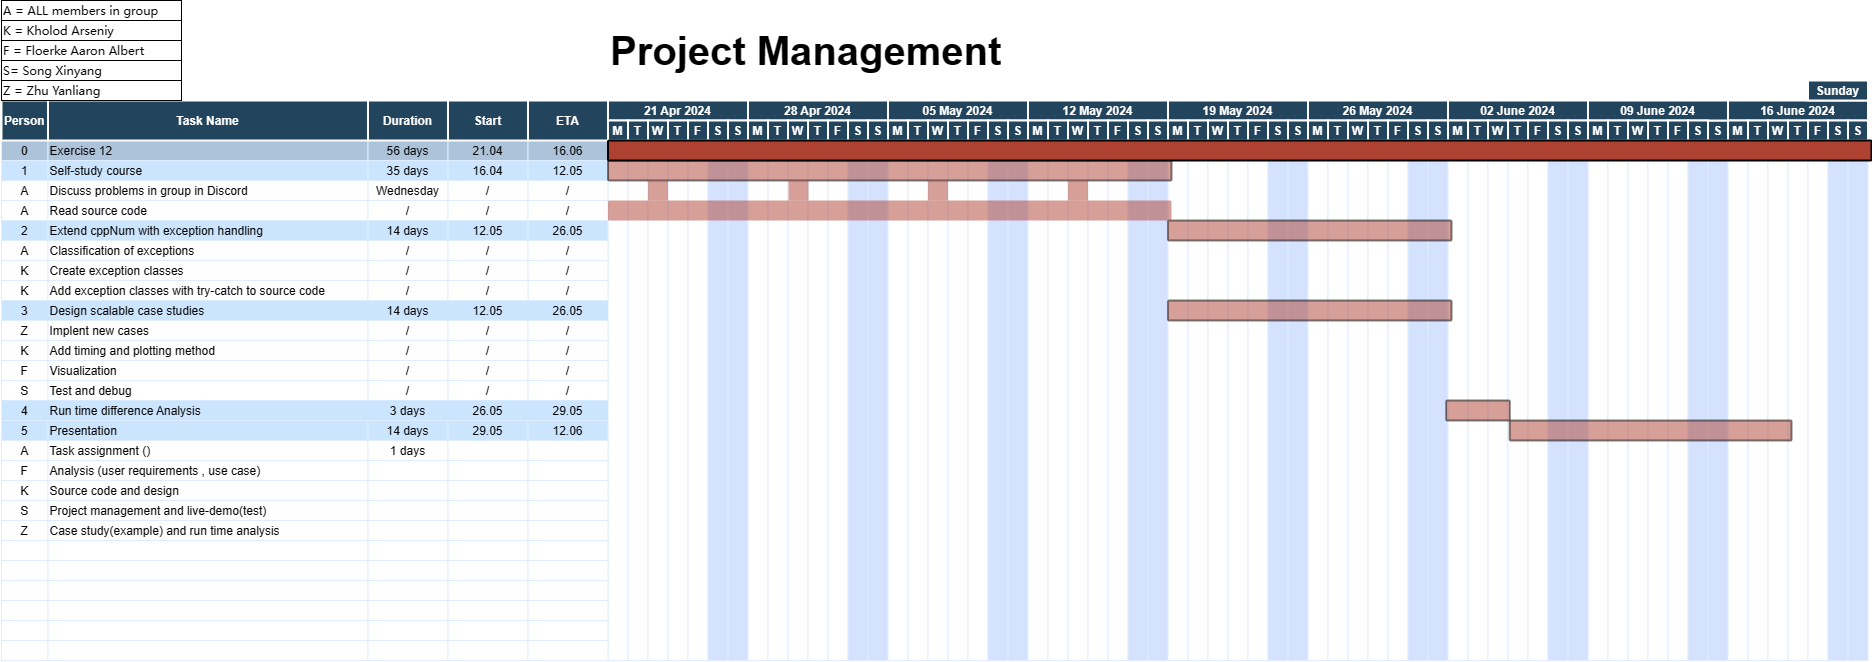
\includegraphics[width=\textwidth]{../project management.png}
    \end{center}
\end{frame}

\begin{frame}
\frametitle{Project Management \\
    \small \color{rwth-blue} Task Assignment}
    
    \begin{flushleft}
        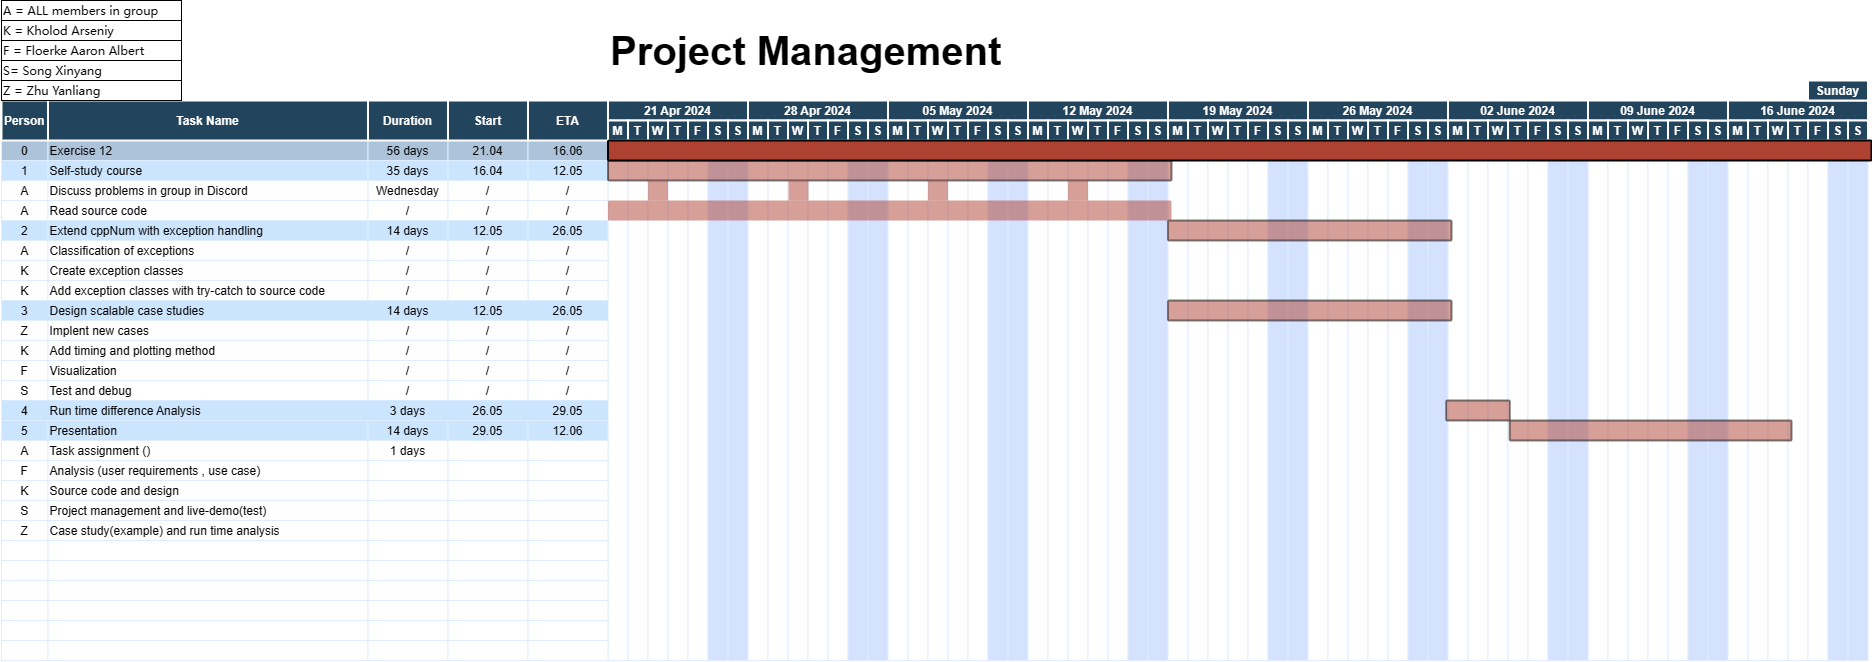
\includegraphics[height=\textheight,keepaspectratio]{../project management.png}
    \end{flushleft}
\end{frame}



\section{Live Software Demo}

\begin{frame}
\frametitle{Live Software Demo \\
	\small \color{rwth-blue} Run in Xubuntu}
	\begin{itemize}	
            \item \textbf{1.Make:}
				\begin{itemize}
				\item make depend
				\item make
				\item make test
				\item make clean
				\end{itemize}
			\item \textbf{2.Execute executable files:}
				\begin{itemize}
				\item ./main.exe + Command-line arguments, (such as testing exception cases).
				\end{itemize}
			\item \textbf{3.Plot:}
				\begin{itemize}
				\item gnuplot gnuplot.plt
				\end{itemize}
	\end{itemize}
\end{frame}



\section{Summary and Conclusion}

\begin{frame}
\frametitle{Summary and Conclusion}
\end{frame}

\end{document}
